\chapter*{Metodyka badań}

\section*{Wprowadzenie do metodyki badań}

Niniejszy rozdział poświęcony jest metodyce badań, mającej na celu zbadanie wpływu tła na klasyfikację obrazów zwierząt przy użyciu zaawansowanych modeli głębokiego uczenia, takich jak ResNet i ConvNeXt. 
Badania te koncentrują się na analizie wyników klasyfikacji przed i po modyfikacjach tła z zastosowaniem różnych metryk oceny jakości, co pozwoli na zrozumienie, w jakim stopniu tło wpływa na wydajność modeli klasyfikacyjnych oraz jakie 
techniki modyfikacji tła mogą być przydatne do poprawy jakości klasyfikacji. W pierwszej części rozdziału zostaną omówione narzędzia i oprogramowanie użyte do badań, konfiguracja sprzętowa oraz biblioteki i frameworki użyte do 
realizacji eksperymentów. Następnie przedstawione zostaną wybrane modele klasyfikacyjne, ResNet i ConvNeXt, wraz z uzasadnieniem ich wyboru oraz krótkim opisem ich architektur i specyfikacji. Kolejna sekcja skupi się na metrykach oceny 
jakości, z wyjaśnieniem, dlaczego właśnie te miary zostały wybrane. Opisany zostanie również zbiór danych wykorzystany w badaniach, jego źródło oraz struktura. Przedstawiony będzię również sposób przygotowania i przetwarzania danych przed 
dokonaniem badań. Kluczowym elementem rozdziału będzie szczegółowy plan przeprowadzenia badań, obejmujący wszystkie etapy, od segmentacji obrazów i usunięcia tła, poprzez modyfikację tła, aż po ocenę wyników modeli przed i po modyfikacjach. 
Dodatkowo, omówione zostaną technikalia implementacji, w tym jak poszczególne etapy zostały zaimplementowane w kodzie, jakie narzędzia programistyczne i techniki kodowania zostały użyte oraz jak zapewniono replikowalność wyników eksperymentów. 
Całość rozdziału zakończy krótkie podsumowanie metodyki badań, co będzie dobrym zakończeniem przed kolejnym rozdzdiałem, w którym omówione zostaną wyniki.

\section*{Przygotowanie środowiska}

Przygotowanie odpowiedniego środowiska badawczego jest kluczowym krokiem w realizacji każdego projektu, szczególnie gdy jest oparty na analizie danych i głębokim uczeniu. W niniejszych badaniach, całość prac została przeprowadzona w języku 
Python, który jest powszechnie stosowany w dziedzinie przetwarzania obrazów i uczenia maszynowego dzięki bogatym zasobom bibliotek i narzędzi wspomagających te dziedziny.

Główne biblitoeki jakie wykorzystano w niniejszych badaniach to: numpy, pandas, scikit-learn, PIL, matplotlib, seaborn oraz torch. Biblioteka numpy została wykorzystana do obsługi operacji numerycznych i manipulacji tablicami, biblioteka 
pandas służyła do manipulacji i analizy danych strukturalnych, głównie do analizy wyników klasyfikacji zapisanych w formacie dataframe. Scikit-learn był wykorzystywany przy obliczeniach metryk i ocenie jakości modeli, a PIL 
(Python Imaging Library) umożliwiła manipulację obrazami i łatwe dokonywanie manipulacji tła. Biblioteki matplotlib i seaborn posłużyły do wizualizacji danych i wyników analiz, co pozwoliło na lepsze zrozumienie uzyskanych rezultatów oraz 
prezentację wyników w przystępnej i zrozumiałej formie.

Kluczowym elementem projektu były wstępnie przeszkolone modele głębokiego uczenia: ResNet, ConvNeXt oraz DeepLabv3. Modele te zostały zaimportowane z biblioteki torchvision, która jest częścią większego ekosystemu PyTorch. Torchvision 
dostarcza łatwy dostęp do przeróżnych wcześniej przetrenowaych modeli na dużych zbiorach danych, co umożliwia efektywne przeprowadzanie eksperymentów bez konieczności trenowania modeli od podstaw na własną rękę i pozwala skupić się na 
najważniejszych aspkektach swoich badań.

Dodatkowo, do analizowania wyników i prowadzenia interaktywnej pracy z kodem, używany był Jupyter Notebook. Jupyter Notebook jest wszechstronnym narzędziem, które umożliwia tworzenie i udostępnianie dokumentów zawierających kod, 
równania, wizualizacje oraz tekst. Jego zastosowanie pozwoliło na przejrzyste prezentowanie procesu badawczego, testowanie i modyfikowanie kodu w czasie rzeczywistym oraz dokumentowanie każdego kroku analizy. Struktura takiego notatnika
składa się z pojedyńczych komórek, co jest bardzo wygodne, jeżeli specyfika naszego badania wymaga poszczególnych wydzielonych funkcjonalności oraz zawiera ciąg przyczynowo-skutkowy.

Całe środowisko badawcze zostało skonfigurowane na lokalnym komputerze wyposażonym w GPU. Korzystanie z GPU było nieocenione dla efektywnego przeprowadzania eksperymentów, zwłaszcza w kontekście obliczeniowo intensywnych operacji związanych z 
przetwarzaniem obrazów i uczeniem maszynowym. W ramach projektu zastosowano system kontroli wersji GIT, a cały kod źródłowy oraz wyniki analiz zostały zapisane i wersjonowane na platformie GitHub. Użycie systemu kontrolii wersji umożliwiło 
efektywne śledzenie zmian w kodzie, co pozwoliło na łatwe zarządzanie i kontrolowanie wersji poszczególnych plików oraz eksperymentów. Dzięki temu każdy etap projektu był dokumentowany, co ułatwiało powrót do wcześniejszych wersji kodu w 
razie potrzeby czy wkradnięcia się błędu. Ponadto, platforma GitHub zapewniła bezpieczne i zorganizowane przechowywanie kodu.

Odpowiednie przygotowanie środowiska z użyciem wymienionych narzędzi i bibliotek było ważnym etapem badania, posiadając dobrze przygotowane środowisko, przeprowadzanie badań zostaje procesem łatwo powtarzalnym oraz wzbogacanie kodu o kolejne 
funkcjonalności również nie będzie przynosić trudności. 

\section*{Wybrane modele}

W niniejszym projekcie zastosowano trzy wcześniej przetrenowane modele głębokiego uczenia: ResNet, ConvNeXt oraz DeepLabv3. Każdy z tych modeli został wybrany ze względu na swoje unikalne właściwości i zdolności do realizacji określonych zadań. 
DeepLabv3 służył jako uniwersalny model do segmentacji, pozwalający na precyzyjne wyodrębnienie obiektów z tła. Modele ResNet i ConvNeXt, o różnych architekturach i z różnymi stopniami zaawansowania technologicznego, zostały wykorzystane do 
klasyfikacji obrazów. ResNet, będący starszym modelem, oraz ConvNeXt, reprezentujący nowsze podejście, zostały wybrane w celu porównania i analizy ich wydajności w kontekście zmodyfikowanych warunków tła. Wykorzystanie gotowych, pretrenowanych 
modeli umożliwiło skupienie się na głównej części badania, jaką jest wpływ tła na klasyfikację obrazów, zamiast na długotrwałym procesie trenowania modeli od podstaw. Poniżej zostanie przedstawiona krótka charakterystyka wykorzystanych modeli,
w celu lepszego zrozumienia kontekstu badania.

\subsection*{ResNet}

ResNet (Residual Network) został zaproponowany w 2015 roku, w którym wygrał wtedy edycję konkursku ImageNet ImageNet Large Scale Visual Recognition Challenge). Bardzo zybko stał się jednym z najpopularniejszych modeli w dziedzinie głębokiego 
uczenia, dzięki swoim szerokim zastosowaniom oraz swoją efektywnością. Główną innowacją ResNet było wprowadzenie residual learning poprzez zastosowanie skrótowych połączeń (skip connections). Pozwala to na efektywne trenowanie bardzo głębokich 
sieci, nawet o setkach warstw, jednocześnie rozwiązując problem zanikania gradientu.

W tradycyjnych sieciach neuronowych, wraz ze wzrostem warst, wzrastał również problem zanikającego gradientu, co znacznie utrudniało efektywne trenowanie modeli. ResNet zaadresował ten problem poprzez wprowadzenie bezpośrednich połączeń 
skrótowych, które umożliwiają przepływ gradientu bezpośrednio przez sieć, omijając kilka warstw pośrednich.

Podstawowym elementem budulcowym ResNet jest blok residual, który może być opisany równaniem:

\begin{equation}
    y = F(x, \{W_i\}) + x
\end{equation}

gdzie \( y \) to wyjście bloku, \( x \) to wejście, a \( F(x, \{W_i\}) \) to funkcja reprezentująca operacje konwolucyjne na wejściu \( x \) z zestawem wag \( \{W_i\} \).

Bloki residual składają się zazwyczaj z dwóch lub trzech warstw konwolucyjnych z dodatkowymi połączeniami skrótowymi, które dodają wejście \( x \) do wyjścia \( F(x, \{W_i\}) \). To skuteczne podejście pozwala na trenowanie bardzo głębokich 
sieci, które byłyby trudne do nauczenia przy użyciu tradycyjnych metod.

ResNet został wybrany do tego projektu ze względu na swoją zdolność do efektywnego radzenia sobie z problemami klasyfikacji, oraz swoją popularność w dziedzinach scztucznej inteligencjii. 

Konkretnym modelem użytym w przeprowadzonych badaniach jest ResNet50. Architektura ResNet50 jest podzielona na cztery główne części: warstwy konwolucyjne, blok tożsamościowy, blok konwolucyjny oraz warstwy całkowicie połączone. 
Schemat architektury tego modelu można zobaczyć na Rys. \ref*{rys:resnet}

Warstwy konwolucyjne w ResNet50 składają się z kilku warstw, po których następuje normalizacja wsadowa (batch normalization) oraz aktywacja ReLU. Warstwy te są odpowiedzialne za ekstrakcję cech z obrazu wejściowego, takich jak 
krawędzie, tekstury i kształty. Następnie warstwy konwolucyjne są uzupełnione warstwami maksymalnego pooling (max pooling), które redukują przestrzenne wymiary map cech, jednocześnie zachowując najważniejsze informacje.

Blok tożsamościowy (identity block) i blok konwolucyjny (convolutional block) są kluczowymi elementami budulcowymi ResNet50. Blok tożsamościowy jest prostym blokiem, który przekazuje wejście przez szereg warstw konwolucyjnych i dodaje wejście z 
powrotem do wyjścia. Pozwala to sieci uczyć się funkcji resztkowych, które mapują wejście na pożądane wyjście. Blok konwolucyjny jest podobny do bloku tożsamościowego, ale z dodatkiem warstwy konwolucyjnej 1x1, która jest używana do redukcji 
liczby filtrów przed warstwą konwolucyjną 3x3.

Ostatnią częścią ResNet50 są warstwy całkowicie połączone (fully connected layers). Warstwy te są odpowiedzialne za przeprowadzenie ostatecznej klasyfikacji. Wyjście z ostatniej warstwy całkowicie połączonej jest przekazywane do funkcji 
aktywacji softmax, aby uzyskać ostateczne prawdopodobieństwa predykowanych klas.

\begin{figure}
	\centering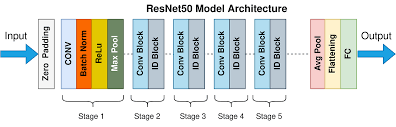
\includegraphics[width=.9\textwidth]{img/resnet.png}
	\caption{Schemat architektury modelu ResNet50}  \label{rys:resnet}
\end{figure}

\subsection*{ConvNeXt}

ConvNeXt to model o nowoczesnej architekturze CNN, który został opracowany w celu integracji najlepszych praktyk z konwolucyjnych sieci neuronowych i nowoczesnych technik pochodzących od transformerów. ConvNeXt wykorzystuje bardziej złożone 
operacje konwolucyjne oraz zaawansowane techniki normalizacji i optymalizacji, co pozwala na osiąganie bardzo dobrych wyników w różnych zadaniach klasyfikacji.

ConvNeXt został zaprojektowany z myślą o zastosowaniu najnowszych technik z dziedziny głębokiego uczenia, takich jak normalizacja warstw (Layer Normalization), mechanizmy uwagi (Attention Mechanisms) oraz bardziej złożone architektury 
warstw konwolucyjnych. W ConvNeXt zastosowano podejście polegające na udoskonaleniu tradycyjnych modułów konwolucyjnych poprzez dodanie elementów inspirowanych transformerami, co prowadzi do lepszej wydajności i efektywności obliczeniowej.

Podstawowym elementem ConvNeXt jest moduł konwolucyjny, który został zoptymalizowany w celu lepszego uchwycenia złożonych wzorców w danych. Architektura ConvNeXt łączy tradycyjne podejścia konwolucyjne z nowymi koncepcjami, co 
prowadzi do lepszej wydajności i efektywności obliczeniowej.

ConvNeXt został wybrany do tego projektu ze względu na swoje nowoczesne podejście i wysoką wydajność w klasyfikacji obrazów, co pozwala na dokładne porównanie z wcześniejszymi modelami state-of-art, takimi jak ResNet.

\subsection*{DeepLabv3}

DeepLabv3 z kolei jest modelem wykorzystywanym do segmentacji obrazów, który został opracowany przez zespół Google. Wykorzystuje on techniki takie jak atrous convolutions (dylatowane konwolucje) i Conditional Random Fields (CRFs), które 
pozwalają na dokładne segmentowanie obiektów na różnych skalach. DeepLabv3+ jest najnowszą wersją tej serii, która łączy atrous convolutions z modulem spatial pyramid pooling, co pozwala na uchwycenie bogatych informacji kontekstowych.

Podstawowym elementem DeepLabv3 jest zastosowanie atrous convolutions, które mogą być opisane równaniem:

\begin{equation}
y[i] = \sum_{k=1}^{K} x[i + r \cdot k] \cdot w[k]
\end{equation}

gdzie \( y[i] \) to wyjście konwolucji, \( x \) to wejście, \( w \) to zestaw wag, \( K \) to rozmiar filtra, a \( r \) 
to współczynnik dylatacji.

Dzięki zastosowaniu atrous convolutions, DeepLabv3 może uchwycić informacje na różnych skalach bez utraty rozdzielczości, co jest kluczowe dla dokładnej segmentacji. Dodatkowo, wykorzystanie spatial pyramid pooling pozwala na 
zbieranie informacji kontekstowych z całego obrazu, co poprawia dokładność segmentacji.

DeepLabv3 został wybrany ze względu na swoją zdolność do precyzyjnej segmentacji obrazów oraz uniwersalnośc użycia, co jest kluczowe dla wyodrębnienia obiektów z tła przed dalszą analizą i klasyfikacją.

\subsection*{Uzasadnienie wyboru modeli}

Wybór ResNet, ConvNeXt oraz DeepLabv3 opierał się na ich sprawdzonej skuteczności w swoich dziedzinach oraz zdolności do realizacji celów tego projektu. ResNet, jako starszy model, pozwala na ocenę wpływu tła na klasyfikację obrazów w 
kontekście bardziej tradycyjnych architektur. ConvNeXt, będący nowoczesnym modelem, reprezentuje najnowsze podejścia i innowacje w dziedzinie głębokiego uczenia, co pozwala na ocenę, jak nowe technologie radzą sobie z problemem tła w porównaniu
do nieco starszych technik. DeepLabv3, jako uniwersalny model segmentacji, umożliwia precyzyjne usunięcie tła, co jest kluczowe dla analiz prowadzonych w ramach tego projektu.

Wykorzystanie gotowych, pretrenowanych modeli pozwoliło skupić się na głównym celu badania – analizie wpływu tła na klasyfikację obrazów – bez konieczności poświęcania czasu na trenowanie modeli od podstaw. Dzięki temu możliwe było 
przeprowadzenie bardziej szczegółowych i kompleksowych badań w zakresie modyfikacji tła i jego wpływu na wydajność modeli klasyfikacyjnych.

\section*{Wybrane metryki}

W celu analizy wyników klasyfikacji przed i po modyfikacjach tła, zastosowano cztery kluczowe metryki: dokładność (accuracy), pewność klasyfikacji (confidence scores), precyzję (precision), recall oraz F1 score. Analizowana będzie również 
macierz korelacji w celu zbadania wzajemnych zależności między modyfikacjami. Metryki te zostały wybrane ze względu na ich zdolność do dostarczania wartościowych informacji na temat wydajności modeli w różnych warunkach, sprawdzają się
one idealnie do wstępnych analiz modeli oraz do oceny jak skutecznie modele radzą sobie z przedstawionym problemem klasyfikacji. Wykorzystane metryki zostaną w tej części krótko opisane. Metryki przeprowadzonych badań będą analizowane 
całościowo, jak również osobno dla każdej klasy, dla każdej różnej modyfikacji tła oraz dla różnych rozmiarów obiektu na obrazie.


\subsection*{Dokładność (Accuracy)}

Dokładność jest jedną z najprostszych i najbardziej intuicyjnych metryk stosowanych do oceny jakości modeli klasyfikacyjnych. Definiuje się ją jako stosunek liczby poprawnie sklasyfikowanych przykładów do całkowitej liczby 
przykładów. Będzie to jedna z głównych analizowanych metryk. Każda klasa będzie posiadała taką samą ilość próbek, także problem interpretowalności tej metryki, jaki występuje przy danych niezbalansowanych nie wystąpi.

Wzór na dokładność prezentuje się następująco:

\begin{equation}
\text{Accuracy} = \frac{TP + TN}{TP + TN + FP + FN}
\end{equation}

gdzie:
\begin{itemize}
    \item TP (True Positives) - liczba prawdziwie pozytywnych przypadków,
    \item TN (True Negatives) - liczba prawdziwie negatywnych przypadków,
    \item FP (False Positives) - liczba fałszywie pozytywnych przypadków,
    \item FN (False Negatives) - liczba fałszywie negatywnych przypadków.
\end{itemize}

Dokładność została wybrana jako podstawowa metryka oceny modeli, ponieważ daje ogólny obraz wydajności modelu.

\subsection*{Precyzja (Precision)}
Precyzja (precision) jest metryką oceniającą dokładność pozytywnych predykcji modelu. Definiuje się ją jako stosunek liczby prawdziwie pozytywnych przypadków do sumy liczby prawdziwie pozytywnych i fałszywie pozytywnych przypadków. 
Wzór na precyzję jest następujący:

\[
\text{Precision} = \frac{TP}{TP + FP}
\]


\subsection*{Recall}
Recall, zwany również czułością lub TPR (True Positive Rate), mierzy zdolność modelu do wykrywania wszystkich pozytywnych przypadków. Jest definiowany jako stosunek liczby prawdziwie pozytywnych przypadków do sumy liczby prawdziwie 
pozytywnych i fałszywie negatywnych przypadków. Wzór na recall 
jest następujący:

\[
\text{Recall} = \frac{TP}{TP + FN}
\]

\subsection*{F1 Score}
F1 score jest harmoniczną średnią precyzji i recall. Jest używany jako pojedyncza metryka oceniająca wydajność modelu, która uwzględnia zarówno precyzję, jak i recall. Wzór na F1 score jest następujący:

\[
\text{F1 Score} = 2 \times \frac{\text{Precision} \times \text{Recall}}{\text{Precision} + \text{Recall}}
\]


\subsection*{Pewność klasyfikacji (Confidence Scores)}

Pewność klasyfikacji (confidence scores) odnosi się do stopnia pewności modelu co do przypisania danego przykładu do określonej klasy. Jest to istotna metryka, ponieważ dostarcza dodatkowych informacji o tym, jak pewny jest model swoich 
predykcji. Wyższe wartości pewności oznaczają większe zaufanie modelu do swojej klasyfikacji.

Analiza pewności klasyfikacji pozwala na ocenę, jak model jest pewny swoich decyzji oraz jak modyfikacje tła wpływają na pewność modeli.

\section*{Opis wykorzystanego zbioru danych}

W ramach niniejszego badania wykorzystano zbiór danych ImageNet1k, który jest jednym z najbardziej rozpoznawalnych i szeroko stosowanych zestawów danych w dziedzinie przetwarzania obrazów i głębokiego uczenia. ImageNet1k składa się z 
obrazów należących do 1000 różnych klas, co pozwala na wszechstronną ocenę wydajności modeli klasyfikacyjnych w różnorodnych scenariuszach.

\subsection*{Struktura zbioru danych}

Zbiór danych ImageNet1k jest podzielony na trzy części: treningową, walidacyjną oraz testową. Każda z tych części ma określoną liczbę obrazów na klasę, co umożliwia wszechstronne trenowanie, walidację i testowanie modeli klasyfikacyjnych.

\begin{itemize}
    \item \textbf{Zbiór treningowy:} Zawiera około 1300 obrazów na klasę, co daje szeroką bazę danych do nauki modeli. 
    Duża liczba obrazów na klasę pozwala na efektywne trenowanie głębokich sieci neuronowych, co prowadzi do lepszego 
    uchwycenia cech charakterystycznych dla każdej klasy.
    \item \textbf{Zbiór walidacyjny:} Składa się z 50 obrazów na klasę. Zbiór walidacyjny jest używany do monitorowania 
    wydajności modelu w trakcie treningu i do wczesnego wykrywania problemów takich jak nadmierne dopasowanie 
    (overfitting).
    \item \textbf{Zbiór testowy:} Zawiera 100 obrazów na klasę. Zbiór testowy służy do ostatecznej oceny wydajności 
    modeli po zakończeniu procesu treningu i walidacji.
\end{itemize}

\subsection*{Różnorodność obrazów}

Obrazy w zbiorze ImageNet1k charakteryzują się różnorodnością rozdzielczości oraz warunków, w jakich zostały wykonane. Inaczej mówiąć, oznacza to, że obrazy mogą przedstawiać obiekty w różnych skalach, oświetleniach, perspektywach i na 
różnych tłach. Taka różnorodność sprawia, że zbiór ImageNet1k doskonale odzwierciedla realistyczne warunki, z jakimi modele mogą się spotkać w praktycznych zastosowaniach. Dzięki temu, modele trenowane na tym zbiorze danych są bardziej 
uniwersalne i mają lepszą zdolność do generalizacji. 

\subsection*{Popularność i znaczenie ImageNet1k}

ImageNet1k jest jednym z najczęściej używanych zestawów danych w badaniach nad różnymi problemami związanymi z głębokim uczeniem, co jest wynikiem jego dużej ilośći zdjęć, różnorodności i realistycznego charakteru. Wiele przełomowych modeli, 
takich jak VGG czy ResNet, zostało przetestowanych i zweryfikowanych przy użyciu tego zestawu danych. Popularność ImageNet1k sprawia, że wyniki uzyskane na tym zbiorze są łatwo porównywalne z wynikami innych badań, co umożliwia ocenę 
postępów i łatwe porównywanie z innymi badaczami.


\section*{Plan badań}

Niniejszy rozdział opisuje szczegółowy plan badań, które zostały przeprowadzone w celu zbadania wpływu tła na klasyfikację obrazów zwierząt. Poniżej szczegółowo przedstawiono kroki podjęte w celu realizacji badań.

\subsection*{Przygotowanie środowiska pracy}

Pierwszym krokiem było przygotowanie odpowiedniego środowiska pracy. W tym celu skonfigurowano środowisko programistyczne, które obejmowało instalację niezbędnych bibliotek i narzędzi, takich jak numpy, pandas, scikit-learn, 
PIL, matplotlib, seaborn, torch oraz torchvision. Przyogotowano również wirtualne środowisko, pobrano dane z oficjalnej strony ImageNet. 

\subsection*{Implementacja}

Całość implementacji została wykonana w języku Python, który dzięki swojej elastyczności i szerokiej gamie bibliotek doskonale nadaje się do realizacji złożonych projektów związanych z uczeniem maszynowym. Większość funkcjonalności została 
zaimplementowana w formie samodzielnych skryptów, podczas gdy same badania, czyli opracowywanie wyników, są dostępne w formie interaktywnych notebooków Jupyter. Taki podział pozwala na łatwe uruchamianie skryptów oraz jednoczesną analizę i 
wizualizację wyników.

Skrypty są nazwane zgodnie ze swoją funkcjonalnością, co ułatwia nawigację i zrozumienie ich przeznaczenia. Każdy skrypt zawiera funkcje z dobrze opisanymi nazwami, a każda funkcja posiada docstringi, które szczegółowo wyjaśniają jej działanie.

Dodatkowo, cała implementacja wraz z dokładnym opisem znajduje się na GitHubie, gdzie można znaleźć pełen kod oraz plik README zawierający instrukcje dotyczące uruchamiania skryptów i analizy wyników. 

Link do repozytorium GitHub: \href{https://github.com/paulpel/BackgroundImpactAnalysis}{link do repozytorium}

\subsection*{Wybranie modeli do segmentacji i klasyfikacji}

Kolejnym ważnym krokiem było zaplanowanie wykorzystywanych modeli w badaniu. Do segmentacji obrazów wybrano model DeepLabv3, który jest zaawansowanym modelem segmentacji zdolnym do precyzyjnego wyodrębniania obiektów z tła. 
Do klasyfikacji obrazów wybrano dwa modele: ResNet, reprezentujący starszą generację modeli głębokiego uczenia, oraz ConvNeXt, będący nowszym i bardziej zaawansowanym modelem. Wybór tych modeli pozwolił na dokładne porównanie ich wydajności 
w kontekście różnych modyfikacji tła oraz dwóch genereacji modeli.

\subsection*{Wybranie klas zwierząt}

Ze względu na ograniczoną dostępność klas w modelu segmentacyjnym DeepLabv3, oraz braku zasobów do analizy wszystkich klas, do badań wybrano 10 zróżnicowanych klas zwierząt. Wybrane klasy były takie, które można skutecznie wysegmentować przy 
użyciu tego modelu. Każda klasa ma przynajmniej jedną zbliżoną do siebie, w celu stworzenia warunków badania sprzyjajązych popełnianiu błędów przez klasyfikatory, przykładowo wybrano trzy rasy psów. Przykładowe zdjęcia dla każdej wybranej 
klasy można zaobserwować na Rys. \ref{rys:classes}

\begin{figure}
	\centering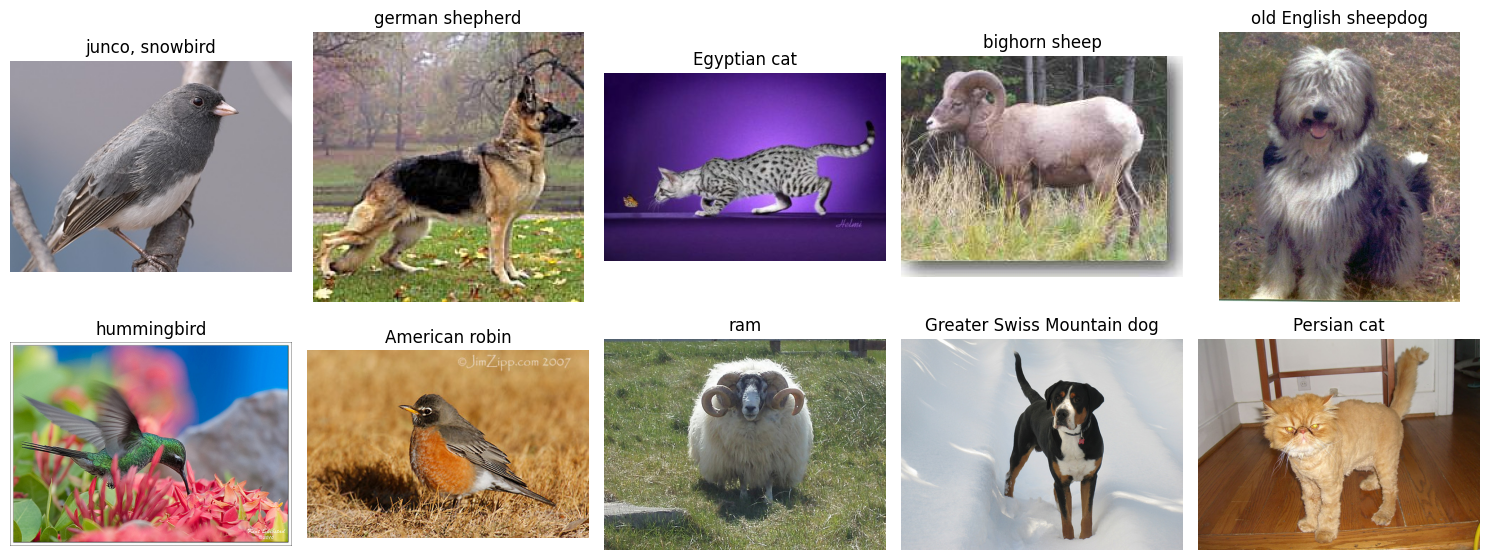
\includegraphics[width=.9\textwidth]{img/classes}
	\caption{Przykładowe oryginalne zdjęcia wybranych klas}  \label{rys:classes}
\end{figure}

\subsection*{Segmentacja obrazów}

Dla każdej z wybranych klas zwierząt wysegmentowano 1000 zdjęć ze zbioru treningowego za pomocą modelu DeepLabv3. Ponieważ na niektórych zdjęciach widniało więcej klas obiektów rozpoznawanych przez ten model, konieczne było zidentyfikowanie 
wartości grayscale dla pożądanej maski obiektu. W tym celu zastosowano skrypt analizujący najczęściej występującą wartość na przestrzeni wszystkich zdjęć dla danej klasy, co pozwoliło na dokładne wyodrębnienie obiektów. Maski zostały zapisane 
do dalszych analiz. Przykładowe uzyskane maski można zaobserwować na Rys. \ref{rys:masks}

\begin{figure}
	\centering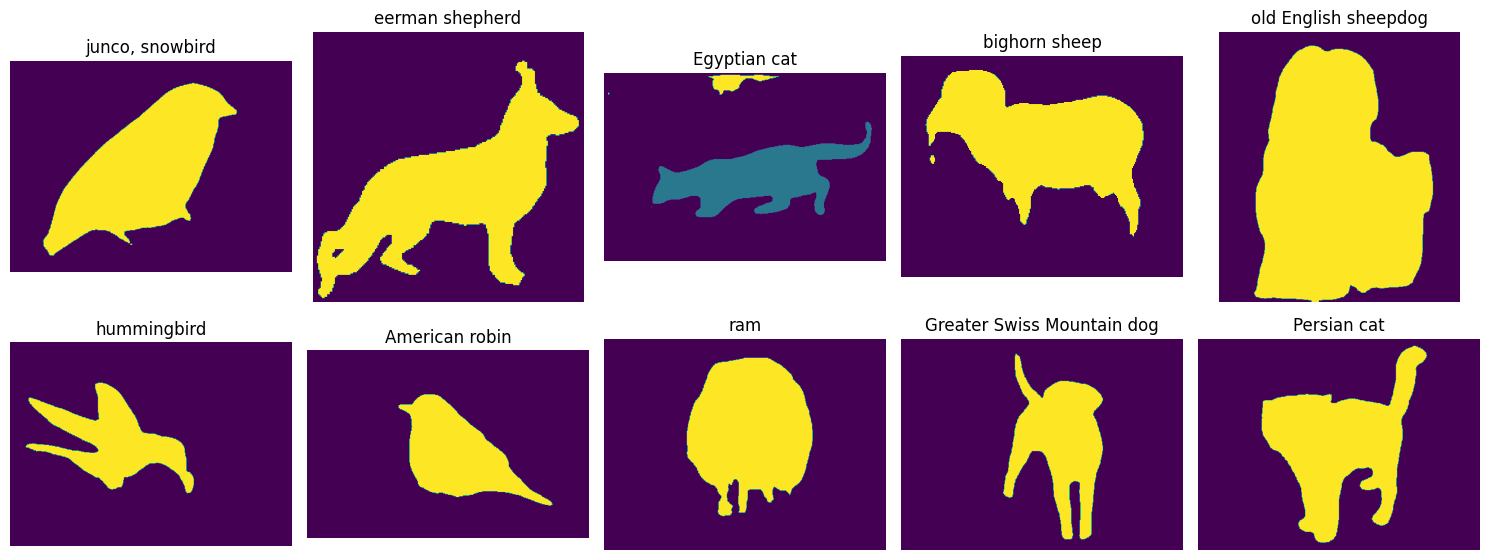
\includegraphics[width=.9\textwidth]{img/masks}
	\caption{Maski przykładowych wysegmentowanych obrazów}  \label{rys:masks}
\end{figure}

\subsection*{Przygotowanie zmodyfikowanych zbiorów zdjęć}

Dla każdej klasy zwierząt przygotowano różne zestawy zmodyfikowanych zdjęć:
\begin{itemize}
    \item \textbf{Zdjęcia z samym obiektem:} Usunięto tło za pomocą maski, pozostawiając czarne tło.
    \item \textbf{Zdjęcia z samym tłem:} Odwrotna modyfikacja do poprzedniej, pozostawiając samo tło bez obiektu. 
    \item \textbf{Przeniesienie obiektu na różne scenerie:} Obiekty zostały przeniesione na inne różne tła o innej scenerii, były to: miasto, pustynia, wnętrze domu, dżungla, góry, niebo, śnieg oraz woda. Ma to na celu stworzenie wariantów 
    zdjęć w innych sceneriach co może być mylące dla klasyfikatorów, szczegónie przy klasyfikacji zwierząt, gdzie podobnie wyglądające gatunki mogą występować w różnych środowiskach. 
    \item \textbf{Zastąpienie tła kolorem o niskim oraz wysokim kontraście do obiektu:} Kolejną modyfikacją było przeniesienie obiektów na tło o kolorze niskokontrastowym oraz wysokokontrastowym. W celu znalezienia tych kolorów, dla każdej klasy 
    przeanalizowano każde zdjęcie i zebrano dominujące kolory dla danej klasy. Następnie przy pomocy specjalnego skryptu wyliczono kolory o niskim i wysokim kontraście do tych obiektów. 
\end{itemize}

Przykładowe zdjęcie, wraz z jego modyfikacjami można zobaczyć na Rys. \ref*{rys:modified}

Modyfikacji dokonywano za pomocą wcześniej uzyskanych masek, dla każdego rodzaju modyfikacji stworzono osobny skrypt w celu zachowania obiektowego charakteru środowiska programistycznego.

\begin{figure}
	\centering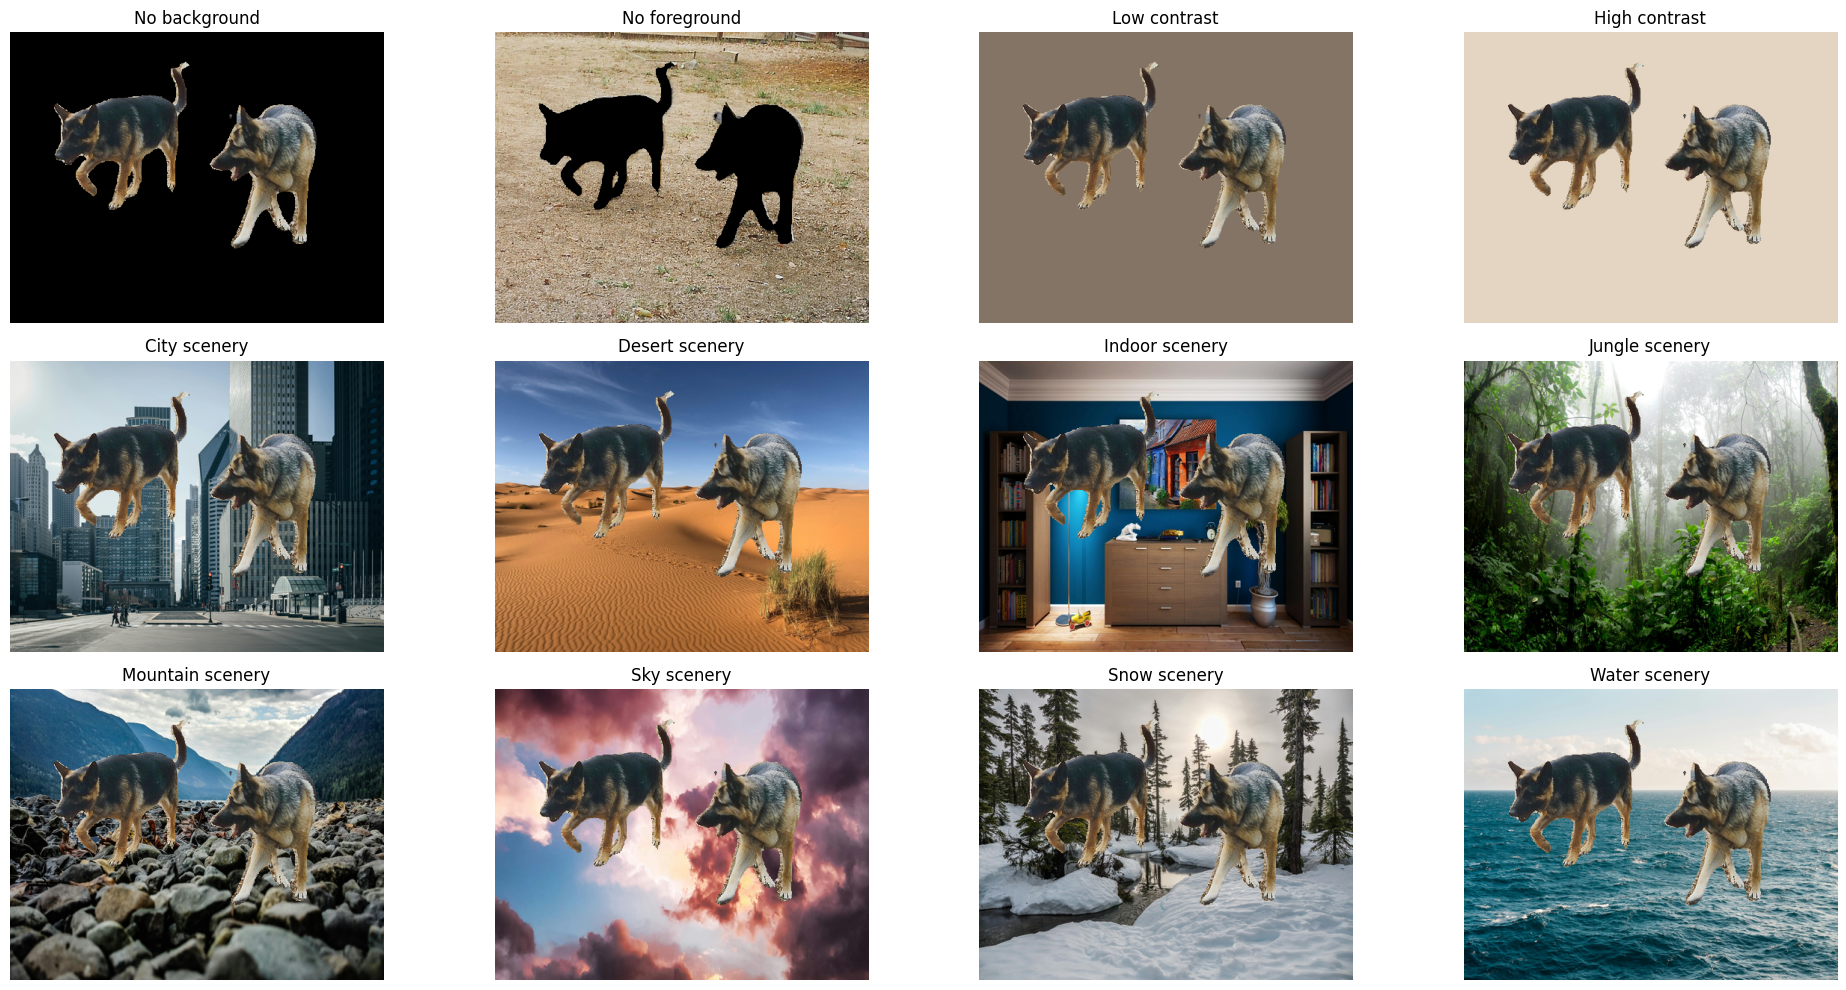
\includegraphics[width=.9\textwidth]{img/modified}
	\caption{Przykładowe zdjęcie poddane modyfikacją}  \label{rys:modified}
\end{figure}

\subsection*{Dokonanie predykcji na wybranych modelach}

Dla każdego zdjęcia dokonano predykcji dla dwóch wybranych modeli, za równo dla oryginalnych zdjęć oraz dla każdego typu modyfikacji. Co dawało dla jednej klasy trzynaście tysięcy predykcji, dwanaście modyfikacji po 1000 zdjęć oraz 
1000 oryginalnych zdjęć. Wyniki predykcji oraz wartości confidence score zapisano w pliku csv.

\subsection*{Dodanie kategorii zdjęć pod względem procentu zajmowanego przez obiekt na zdjęciu}

Zbadanie stosunku wielkości obiektu do całego zdjęcia jest istotne w kontekście badania wpływu tła na klasyfikację, ponieważ może znacząco wpływać na wyniki modeli klasyfikacyjnych. Wielkość obiektu w stosunku do tła może determinować, 
jak łatwo model jest w stanie rozpoznać i sklasyfikować obiekt. Mniejsze obiekty mogą być trudniejsze do wykrycia i bardziej podatne na zakłócenia ze strony tła, podczas gdy większe obiekty mogą dominować obraz, co ułatwia ich klasyfikację. 
Analiza wpływu różnych procentyli wielkości obiektu pozwala na zrozumienie, w jakim stopniu tło oddziałuje na modele w zależności od proporcji obiektu na zdjęciu, co z kolei może prowadzić do bardziej efektywnych strategii przetwarzania i 
klasyfikacji obrazów w praktycznych zastosowaniach.

Dla każdego zdjęcia dodano kategorię pod względem procentu zajmowanego przez obiekt na zdjęciu. Przykładowe zdjęcia o różnych 
rozmiarach obiektów można zobaczyć na Rys. \ref*{rys:size_comp}

\begin{enumerate}
    \item \textbf{Obliczenie powierzchni obiektu:} Dla każdego obrazu obliczono liczbę pikseli zajmowanych przez obiekt.
    \item \textbf{Obliczenie powierzchni całkowitej obrazu:} Liczba pikseli całego obrazu.
    \item \textbf{Obliczenie procentu powierzchni zajmowanej przez obiekt:} Procent powierzchni zajmowanej przez obiekt obliczono za pomocą wzoru:
    \begin{equation}
    \text{Procent powierzchni zajmowanej przez obiekt} = \left( \frac{\text{Powierzchnia obiektu}}{\text{Powierzchnia całkowita obrazu}} \right) \times 100
    \end{equation}
    \item \textbf{Podział obiektów na percentyle:} Obrazy posortowano według procentu powierzchni zajmowanej przez obiekt i 
    podzielono na trzy grupy według wartości percentyli (0,33 oraz 0,66) i nadano każdemu zdjęciu odpowiednią kategorie (SMALL, MEDIUM albo LARGE)
\end{enumerate}

\begin{figure}
	\centering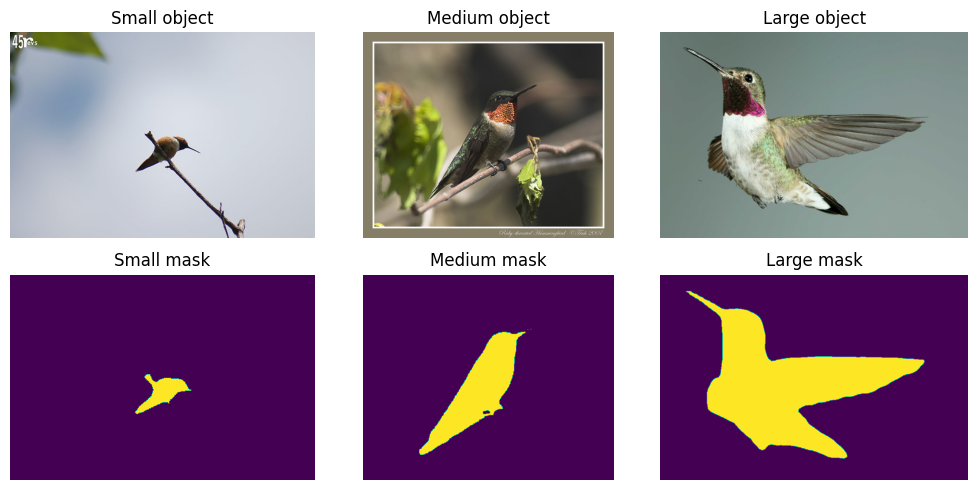
\includegraphics[width=.9\textwidth]{img/size_comp}
	\caption{Przykładowe zdjęcia o różnych rozmiarach obiektów dla klasy "hummingbird"}  \label{rys:size_comp}
\end{figure}

\subsection*{Analiza wyników}

Wygenerowany plik csv załadowano do dataframe, następnie przygotowoną tą ramkę w celu dalszych analiz. Dodano informacje o prawdziwej klasie do każdego zdjęcia oraz informacje True, False w zależnośći od poprawności klasyfikacji dla każdej 
modyfikacji. Ułatwiło to dalsze generowanie statystyk i metryk. Analizy wyników dokonano ze względu na różne czynniki, wymienione poniżej:
\begin{itemize}
    \item \textbf{Analiza ogólna wyników:} Ogólna wydajność modeli na całym zbiorze danych.
    \item \textbf{Analiza pod kątem wielkości obiektu:} Wydajność modeli w zależności od wielkości obiektu na zdjęciu.
    \item \textbf{Analiza pod kątem rodzaju modyfikacji:} Wydajność modeli w zależności od typu modyfikacji tła.
    \item \textbf{Analiza pod kątem klasy:} Wydajność modeli dla każdej klasy zwierząt osobno.
\end{itemize}

\subsection*{Wnioski i dalsze kierunki rozwoju}

Kolejnym etapem badania było wyciągniecie wniosków na podstawie uzyskanych rezultatów oraz przedstawienie potencjalnych kierunków rozwoju projektu.
